\documentclass[11pt,twocolumn]{article}
\usepackage[utf8]{inputenc}
\usepackage{graphicx}



\graphicspath{}

\author{
  \texttt{Sebastian Bångerius}
  \and
  \texttt{Villiam Rydfalk}
}

\begin{document}
\pagenumbering{gobble}

\title{Multi-path throughput in mobile networks}
\maketitle

\cleardoublepage


\section{Abstract}

We have made a project about the throughput in multipath networks. Specifically in WiFi and Bluetooth networks. By analysing and comparing these we have made a few conclusions about strengths and weaknesses for both. We have done a simulation of some scenarios based on the real world and what might happen in a network. We had some hypothesis about what should happen in these scenarios and discussed possible solutions. Once we conducted the simulations we revised our hypothesis and made an analysis of the results. We came to a conclusion and discussed other possible scenarios. We have also made some hypothesises about when and where the different methods of network routing should be used and a few examples of implementations.

\section{Introduction}

The way we transfer information varies a lot between places and situations. Some techniques work better in certain environments, while they encounter complications in others. People in different countries have different interests, standards and financial potential. Because of all these circumstances affecting mobile networks, it is important to actually study how information flows through them. For instance; in areas with high population density there might be easier to rout data between end users towards an access point, while in sparsely populated areas it might be better with one cellular tower (or even a satellite) for connection. In a lot of central and southern African countries people have access to a phone but no electricity, in such an environment power saving might be a key feature of data transfer, and some power consuming routing options are excluded.

There are many ways to transfer information electronically, however in this report we will focus on routing in different kinds of networks and different methods of routing. In many networks there is a lot of data flowing and the traffic is very high over certain paths. If a path is faster than other then many protocols will try to use that path even though it is heavily burdened since it is hard to measure traffic until after a packet has failed to be delivered. So one way to solve this is by sending a few packets over a different path even though it is slower. This is referred to as multipathing. The theory is that by sending packets different routes the throughput and effective use of the network will be higher than if the devices send all packets the same route. 


\section{Method}

We want to evaluate different methods of pathing in a network to get good throughput. If we are to do any tests on a larger scale it will be a lot of complex work unless we do a simulation. Since we want to do tests based on multipathing, the simulator has to include a few features. These will be briefly discussed in the following paragraph.

First of all we need a few nodes that can connect in a way we want, and they have to be able to communicate with a given quantity of data that we can measure. We also need to be able to split this data up in any way we want between several paths. In these paths we have to be able to set different factors like noise, other traffic and just about anything that would interfere with our packets in a "real world" scenario.

Once we have software that can do all this we have a few experiments we will try. At first we will just test the most simple networks with only a few nodes sending data to each other without any real interference to get a sense of what is good throughput and a calm network. Once we have done this we will raise the complexity of the network. Add more nodes that communicate with each other and flooding the network with packets. Our hope is to be able to do this as gradually as possible to see the decline in effectiveness of the network. Hopefully we will be able to see a trend of what factors do the most good or harm to the network and what methods of routing are best for each different scenario.
\begin{figure}[ht]
\begin{center}
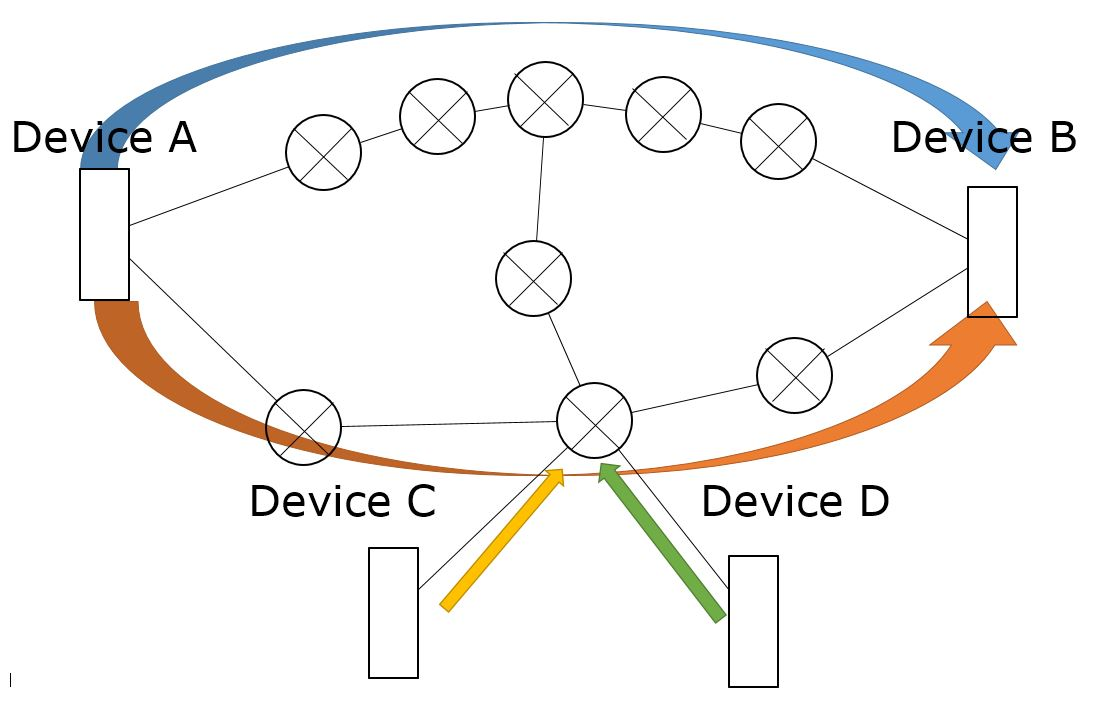
\includegraphics[scale=0.26]{Figure_1}
\end{center}
\end{figure}


\section{Hypothesis}

When it comes to networks in the real world there will be a lot of different types and some won't have the same problems. But in ad-hoc networks where there is a lot of information to be sent between the nodes there will be a lot of traffic, and a lot of burdening on some paths since there will always be one path that is faster than another.

With the test we are going to do evaluate weather multipathing helps a network to get a higher throughput or not. Our guess is that it will improve the performance of the network and here is why:

When a path is used very heavily then the traffic there might collide and cause dropped packets. This will result in delays and more traffic back and forth. This could be avoided if the nodes were to use 2 or 3 of the fastest routes instead of just the single fastest one. If the network is not very burdened then this might be a waste of time since it might take longer for the data to arrive than if it sent all over the same fast path, but in a network with a lot of users and a lot of traffic it might improve the chance of a stable line of communication.

Also, when there is a lot of different paths there is less chance of trouble if one path would be broken since you already have a few other paths saved. If you simply used one path you would now have to search for a new one before being able to send the rest of your data.

There are still some problems with multipathing. When looking at multipathing between cellular and wi-fi (which is probably the most relevant multi-channel implementation) we can often see a significant difference in RTT (round trip time). We believe that this might end up showing some interesting effects in the case of multipathing. We also often have the issue of the cellular connection being metered, which is a strong reason to not use it if wi-fi is available. These two facts lead us to believe that there are ways to use the multipathing in such a way that both links are able to bring their respective benefits into the multipathing algorithms. One might be able to distribute the data over the two links depending on some attribute of the data, for instance how big the packet is or what application requested the TCP-delivery. Though the latter suggestion will probably violate the protocol stack praxis.


\section{Time plan}
\begin{description}
\item[Week 38]
Acquire information about how packets flow through different network types. Get a more detailed plan.
\item[Week 39]
Write ~2 pages. Find and learn tools for network simulation. Complete milestone 2
\item[Week 40]
Write ~2 more pages (so ~4 in total). Make first trial simulations
\item[Week 41]
Write ~3 more pages (so ~7 in total). Make sharp simulation. Draw conclusions. Make beautiful diagrams in Excel. Drool over said diagrams.
\item[Week 42]
Seminar and finish report
\end{description}



\end{document}